We will begin by outlining the objectives for our automation of the data analysis:

\begin{enumerate}
  \item All produceables are called via a {\tt Makefile}.
  \item Data is imported from an online public storage site.
  \item Energy calibration is completed on at least one isotope from the energy data.
  \item The lab report is written in \LaTeX and complied via the make file into a .pdf document
  \item All files are pushed to {\tt GitHub} for submission.
\end{enumerate}

Each of one these tasks will provide insight into data analysis, technical writing, and
production of publishable documents.

\subsection{Peak Fitting}

As the importing of data is a routine exercise, we will start with the discussion of our analysis in Python.
The first task is to read and unpack the data file and convert it to a {\tt numpy} array. From this array, we will parse the data and
build sub arrays for each isotope. We then manually input the known gamma energy for each isotope. These known values are shown below, as well
as a composite spectrum of all the sources.

\begin{figure}[h]
  \begin{center}
      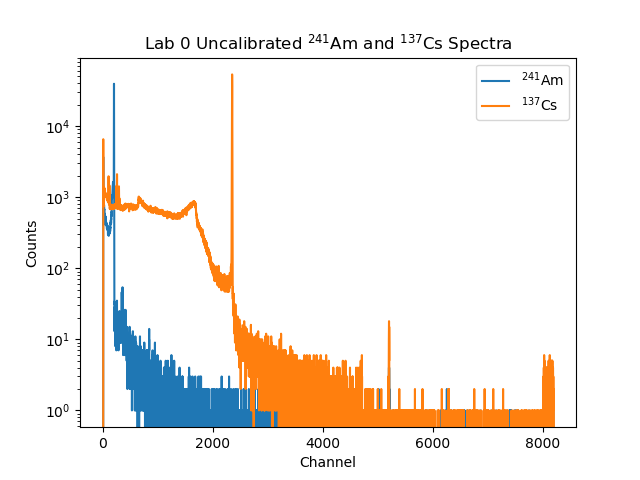
\includegraphics[width=7cm]{am_cs_uncalibrated.png}
      \caption{\label{fig:uncal_spec}Uncalibrated Spectra for $^{241}$Am and $^{137}$Cs }
  \end{center}
\end{figure}

Once the peak values are assigned, we then determined the indexing of this known value within the data for several peaks.
Now knowing the difference between the binned energy and the published energy, you can calibrate the rest of the spectrum based
on this difference.

\begin{figure}[h]
  \begin{center}
      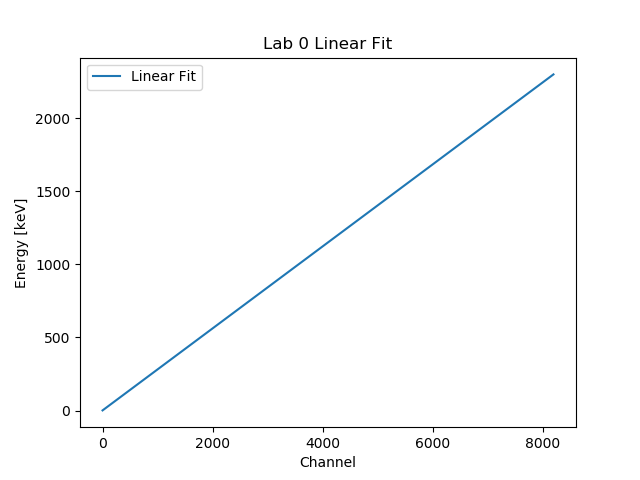
\includegraphics[width=7cm]{linear_fit.png}
      \caption{\label{fig:linear_fit}Linear fit model for spectra}
  \end{center}
\end{figure}


When we apply this fit to the data and you can clearly see the 662 keV peak of $^{137}$Cs is properly calibrated.

\begin{figure}
  \begin{center}
    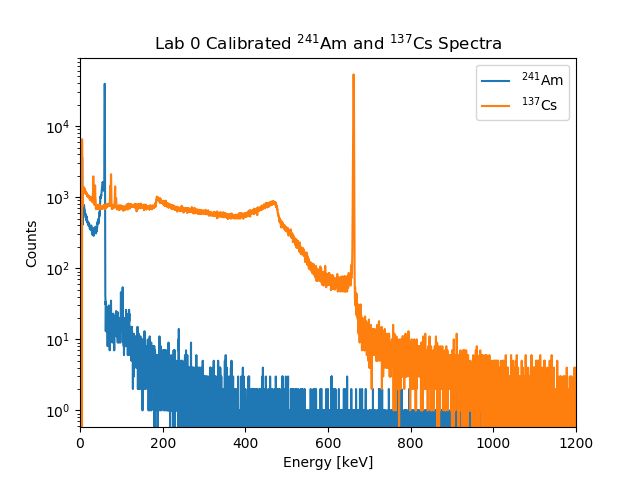
\includegraphics[width=10cm]{am_cs_calibrated.png}
    \caption{\label{fig:uncal_spec2}Uncalibrated Spectra for $^{241}$Am and $^{137}$Cs }
  \end{center}
\end{figure}
